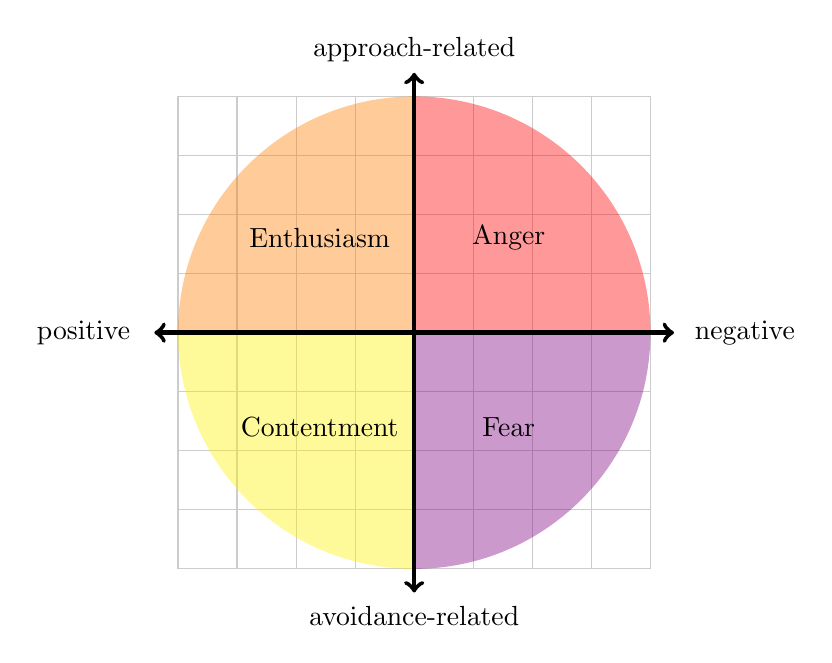
\begin{tikzpicture}[scale=3]
		\draw[step=0.25,black,thin,opacity=0.2] (-1,-1) grid (1,1);
		
		\fill [red, opacity=0.4] (1,0) arc [radius=1,start angle=0,end angle=90] -- (0,0);
											   
		\fill [violet, opacity=0.4] (0,-1) arc [radius=1,start angle=270,end angle=360] -- (0,0);
		
		\fill [orange, opacity=0.4] (0,1) arc [radius=1,start angle=90,end angle=180] -- (0,0);
		
		\fill [yellow, opacity=0.4] (-1,0) arc [radius=1,start angle=180,end angle=270] -- (0,0);
									   
		%\fill [violet, opacity=0.3] (0.95,-0.95) rectangle (0,0);
		%\fill [orange, opacity=0.5] (-0.95,0.95) rectangle (0,0);
		%\fill [yellow, opacity=0.5] (-0.95,-0.95) rectangle (0,0);
		
		\draw [ultra thick, <->] (-1.1,0) --(1.1,0);
		\draw [ultra thick, <->] (0,1.1) --(0,-1.1);
		\node at (0.4,0.4) {Anger};
		\node at (0.4,-0.4) {Fear};
		\node at (-0.4,0.4) {Enthusiasm};
		\node at (-0.4,-0.4) {Contentment};
		
		\node at (1.4,0) {negative};
		\node at (-1.4,0) {positive};
		\node at (0,1.2) {approach-related};
		\node at (0,-1.2) {avoidance-related};
	\end{tikzpicture}